\documentclass{article}
\title{高校物理やり直し — 力とエネルギーから電気まで}
\author{TeX 図書館}

\begin{document}

\section{読み方 — この本の地図と 3 つの道具}

高校物理でつまずくポイントは、ほぼ 1 か所に集約されています。\textbf{「式を暗える前に、物体の運動の絵が描けていない」}こと。物理の問題は、まず「今、何がどう動いていて、力はどこからどちら向きに働いているか」を絵に描けば半分解けたも同然です。絵が描けないまま式だけを覚えると、「どの公式を使えばいいのか」が毎回思い出せなくなります。この本は、絵を先に描き、式を後から載せる順番でやり直す本です。

もう 1 つのつまずきは、\textbf{単位とベクトルの 2 つの道具を軽視すること}です。速さと速度の違い、グラムとキログラムの違い、そうした細かい部分が後半の電気や波で一気に効いてきます。だから最初の 2 節で、この 2 つの道具をきちんと手に入れてから先へ進みます。

\subsection{全 10 節の見取り図}

節の配分は次のとおりです。

\begin{enumerate}
\item 第 1 節: 読み方。この本の方針と道具を決めます。
\item 第 2〜3 節: 速さと等加速度運動。動き出す物体の絵を描きます。
\item 第 4 節: 力と運動。ニュートンの 3 法則がすべての中心です。
\item 第 5〜6 節: エネルギーと運動量。運動の「量」を 2 通りに数えます。
\item 第 7〜8 節: 波と音・光。揺れが伝わる様子を扱います。
\item 第 9 節: 電気と回路。電子の流れを水にたとえて読みます。
\item 第 10 節: まとめと次の一歩。
\end{enumerate}

各節の終わりには\textbf{解答の指針}を置きます。答えの丸写しではなく、どの絵を描き、どの式を立てるかを書く欄です。まず自力で 5 分考えてから、その欄を開いてください。

\subsection{本書で最初に使う式は 2 つだけ}

等加速度直線運動の道具は、次の 2 つに絞ります。勝手な公式を増やしません。加速度とは「1 秒ごとに速度がどれだけ変わるか」でした。だから \( n \) 秒後の速度は、初めの速度に加速度分を足すだけです。

\[ v = v_{0} + at \]

もう 1 つは、変位(進んだ距離)です。速度がグラフに描けることは第 3 節で詳しくやりますが、前半の道具として先に載せておきます。

\[ x = v_{0} t + \frac{1}{2} a t^{2} \]

\begin{quote}
\textbf{【注意】}\ 単位と向きは式と一緒に書くこと。速度の単位は m/s、加速度の単位は m/s\(^{2}\) であり、両者は別の目盛りです。また、この 2 式は\textbf{向きが決まっている量(ベクトル)}を扱います。右向きを正にする、上向きを正にする、と問題ごとに 1 行書いてから立式すると、符号のミスがほぼなくなります。
\end{quote}

\textbf{解答の指針:}\ まず問題文から「何の時点の、何を求められているか」を日本語で 1 行書く(例: 発射 2 秒後の速度)。次に、右向き正など向きの取り方を決める。最後に、初速度・加速度・時間のうち既知のものを書き出してから式を選ぶ。既知の量を書き出す前に公式を選ぶのが、つまずきの最大の原因です。

\section{速さと速度 — 「はやさ」と「向き」を分ける}

最初につまずきやすいのが、速さと速度の違いです。日常では同じ言葉に聞こえますが、物理では明確に分けます。\textbf{速さは「どれだけはやいか」だけ。速度は「どちら向きに、どれだけはやいか」まで言う}言葉です。

例えば、トラックが一周して出発点に戻ったとします。走った道のり(実際に動いた道の合計)は例えば 400 m ですが、出発点に戻ってきたので、始点と終点を結ぶ\textbf{変位}は 0 です。このとき平均の速さは 400 m を時間で割った値ですが、平均の速度は 0 になります。道のりと変位の違い、これが速さと速度の違いの中身です。

\subsection{ベクトルとスカラー}

量を 2 種類に分けて整理しておきます。

\begin{itemize}
\item \textbf{スカラー(向きがない量)}: 道のり、時間、質量、速さ、温度。
\item \textbf{ベクトル(向きがある量)}: 変位、速度、加速度、力。
\end{itemize}

ベクトルは「大きさと向き」で決まります。紙の上では矢印で描きます。矢印が同じでも「右向き 5 m/s」と「左向き 5 m/s」は別の速度です。計算では、どちら向きを正にするかを最初に宣言します。右を正と決めたら、左向きの量はすべてマイナスの符号で書きます。こうすると、ベクトルの計算は普通の足し算・引き算に戻ります。

\subsection{平均と瞬間}

車のメーターが示しているのは\textbf{瞬間の速さ}です。一方、走行距離を移動時間で割ったのは\textbf{平均の速さ}です。渋滞で止まっていた時間も含めると、平均の速さはメーター表示よりずっと小さくなります。この 2 つが別物であることは、計算問題でもよく問われます。

平均の速度は、変位を時間で割って求めます。

\[ \bar{v} = \frac{x}{t} \]

逆に、速さが一定の間は「距離 = 速さ × 時間」がそのまま使えます。単位に注意してください。時速 72 km は、72 km ÷ 3600 s を計算して秒速 20 m です。km/h と m/s の換算は、\textbf{m/s に直すには 3.6 倍、km/h に直すには 3.6 で割る}と覚えておくと速いです。

\begin{quote}
\textbf{【注意】}\ 「速度が 0 でも加速している」場面はあります。頂点に来たボールは、瞬間的に止まっていますが、すぐに落下し始めます。つまり速度は減り続けて 0 を通り越して増えているので、頂点でも加速度は下向きに働き続けています。「止まっている = 力が釣り合っている」ではありません。
\end{quote}

\textbf{解答の指針:}\ 「速さ」が聞かれているのか「速度」が聞かれているのか、問題文で太字の部分を意識して区別する。道のりを使うか変位を使うかの違いにすぎません。次に、与えられた単位が km/h か m/s かを確認し、そろっていなければ 3.6 倍・3.6 分の 1 でそろえる。最後に、向きを含む量を足すときは符号をそろえてから計算します。

\section{等加速度直線運動 — 式 3 つは 1 つのグラフから}

一定の力で押し続けられた物体は、一定の割合で速くなります(または遅くなります)。この「速度の変化が一定」の運動を\textbf{等加速度直線運動}と呼び、高校物理の計算問題の半分はここから出ます。しかし公式を 3 つ暗えすれば済む話ではありません。\textbf{1 つのグラフを描けるようになれば、3 つの公式は全部読み取れる}からです。

\subsection{v-t グラフの読み方}

縦軸に速度 \( v \)、横軸に時間 \( t \) を取ったグラフを考えます。初速度 \( v_{0} \)、加速度 \( a \) の等加速度運動は、このグラフ上で直線になります。傾きが \( a \) です。

このグラフには 3 つの情報が詰まっています。

\begin{itemize}
\item \textbf{傾き} = 加速度。急なほど、速く速度が変わっている。
\item \textbf{縦軸との交点} = 初速度。
\item \textbf{グラフと横軸の間の面積} = 変位(進んだ距離)。
\end{itemize}

面積が変位になるのは、「速さ × 時間 = 距離」が一定のときの話を、速度が変わる場面に細切れに適用した合計だと考えれば自然です。台形の面積の公式を書けば、変位の式がそのまま出てきます。

\begin{figure}
\centering
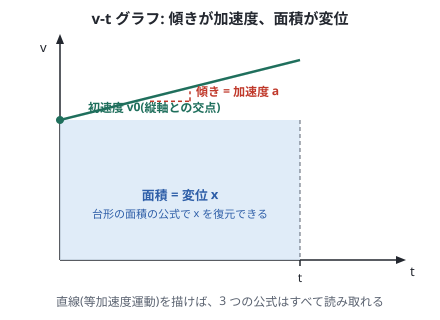
\includegraphics[width=0.85\textwidth]{figures/vt-graph.svg}
\caption{v-t グラフ: 傾きが加速度、面積が変位}
\end{figure}

\subsection{3 つの公式は使い分けではない}

ここから、よく使う形を 3 つ書いておきます。どれも上のグラフから読み取れるものです。

\[ v = v_{0} + at \qquad x = v_{0} t + \frac{1}{2} a t^{2} \qquad v^{2} - v_{0}^{2} = 2ax \]

3 つ目の式は、前の 2 つから時間 \( t \) を消去した形で、「時間が分からないが、速度と距離から加速度を知りたい」場面で役立ちます。大切なのは\textbf{公式を 3 つ暗えることではなく、グラフが描ければ必要な式は導ける}という感覚です。試験中に忘れても、グラフから台形の面積を書けば復元できます。

\subsection{自由落下と垂直投げ上げ}

地面に向かって落とした物体は、重力によって毎秒約 9.8 m/s ずつ下向きの速度が増します。この \( g = 9.8 \) m/s\(^{2}\) を\textbf{重力加速度}と呼びます。質量が違っても同じ加速度で落ちる、というのが驚きのポイントです(重いほうが速く落ちる、というのは空気の抵抗があるときの錯覚です)。

上向きに投げた物体も同じです。上向き正と決めれば、加速度は \( -g \) で一定。速度は毎秒 9.8 m/s ずつ減り、頂点で 0 になり、そのあと下向きに増えていきます。第 2 節の注意で書いたとおり、頂点でも加速度は下向きに \( g \) のままです。

\begin{quote}
\textbf{【注意】}\ 「静止していた物体が動き始める」「動いている物体が止まる」どちらも\textbf{加速度を持つ瞬間}です。速さが変わらない運動(等速直線運動)のときだけ、加速度は 0 です。
\end{quote}

\textbf{解答の指針:}\ まず v-t グラフの見取りを頭に描き、初速度・加速度・時間・変位のうち「分かっているもの」「求めるもの」を表に書く。分かっている量が 3 つあり、求める量が決まれば、3 つの公式のうち使える 1 つが自然に決まります。落体の問題では、上向き正か下向き正かを最初に 1 行書く。頂点は「速度 0、加速度 \( -g \)」と暗記してしまって問題ありません。

\section{力と運動 — ニュートンの 3 法則がすべて}

力とは何か。物理では\textbf{物体の運動を変える働き}のことです。動かし続ける力ではありません。この区別が、つまずきの最大の分かれ目です。

日常の感覚では「動かし続けるには力が要る」ように感じます。実際、床を滑る荷台は勝手に遅くなります。しかし遅くなるのは\textbf{摩擦という力が逆方向に働いているから}で、力がなければ等速で動き続けます。宇宙船がエンジンを切っても飛び続けるのはこのためです。ニュートンはこの「何もしなければ、動くものは動き続ける」性質を\textbf{慣性}と名付けました。

\subsection{運動の 3 法則を言葉で押さえる}

\begin{enumerate}
\item \textbf{第一法則(慣性の法則)}: 力が働かなければ、静止は静止し続け、等速直線運動はそのまま続く。
\item \textbf{第二法則(運動方程式)}: 力の合計が質量と加速度をつなぐ。\( F = ma \)。
\item \textbf{第三法則(作用・反作用)}: A が B に力を加えれば、B は A に同じ大きさ・逆向きの力を返す。
\end{enumerate}

第二法則の \( F = ma \) は、この本の中心です。読み方は「力 \( F \) を加えると、質量 \( m \) の物体が加速度 \( a \) で動き始める」。同じ力でも、質量が大きいほど加速しにくい(重いものは動かしにくい)ことを式が言っています。

第三法則でよく混乱するのは「同じ大きさの力が返ってくるのに、なぜ動くのか」。答えは、\textbf{作用と反作用は別々の物体に働く}からです。床を蹴る力は私を加速させ、床が返す力も私に働きます。しかし前に進めるのは、私が\textbf{床を}蹴るからではなく、摩擦が\textbf{私に}働くから。足が後ろへ滑らなければ、床は私に前向きの摩擦を与えます。相手が別なら、力の足し算をしてはいけません。

\subsection{力のつり合いと運動方程式}

物体が加速度 0 で動いている(または静止している)とき、力の合計は 0 です。これを\textbf{つり合い}と呼びます。つり合いは \( a = 0 \) の運動方程式にすぎません。

加速度があるときは、運動方程式を立てます。手順は決まっています。

\begin{enumerate}
\item 物体を 1 つ選び、図から\textbf{切り離して}描く(対象を明確にする)。
\item その物体に働く力を\textbf{すべて}矢印で書き込む。重力・垂直抗力・摩擦・張力・外から押す力。
\item 動く向きに沿って正の向きを決め、力を足して \( F = ma \) に代入する。
\end{enumerate}

\begin{figure}
\centering
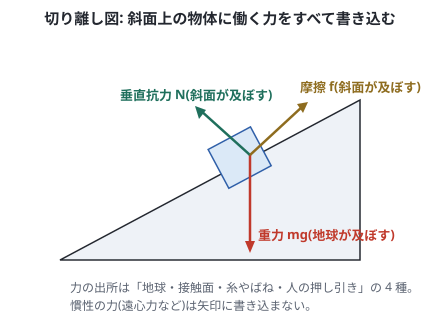
\includegraphics[width=0.8\textwidth]{figures/force-diagram.svg}
\caption{力の図: 斜面上の物体に働く力をすべて書き込む}
\end{figure}

\begin{quote}
\textbf{【注意】}\ 「慣性の力」を矢印に書き込まないこと。運動方程式は「実際に働く力」の合計を右辺に置く式で、遠心力のようないわゆる見かけの力は、別の視点(加速して観察している視点)の話です。最初のうちは「働く力は重力・接触・ばね・電磁気だけ」と数えて、書き漏らしと書きすぎの両方を防ぐのが安全です。
\end{quote}

\textbf{解答の指針:}\ 運動方程式の問題では、切り離し図を描く前に答えを書こうとしない。力を数えるときは「地球(重力)・床や壁(垂直抗力・摩擦)・糸やばね(張力・弾性力)・人の押し引き」の 4 出所を順に確認する。糸でつながった複数の物体なら、物体ごとに式を立てて連立する。斜面の問題では、軸を斜面に沿って取ると計算が簡単になります。

\section{仕事とエネルギー — 労力の貯金箱}

\( F = ma \) は強力ですが、速度が複雑に変わる問題(曲がる・上下する・途中で力が変わる)では式が立てにくくなります。そこで登場するのが\textbf{エネルギー}の考え方です。「力がどれだけ働いたか」を、経路ではなく\textbf{結果(速度と高さ)だけで}数えます。

\subsection{仕事の定義}

物理の\textbf{仕事}は、「力 × その力の向きに進んだ距離」です。単位は J(ジュール)。

\[ W = Fx \]

日本語の「仕事」より狭いことに注意してください。重い荷物を持ち上げてその場でじっと立っていても、重力の向きに動いていないので物理の仕事は 0 です。荷物を水平に運ぶとき、手が荷物に加える力は上向きで、移動は水平。これも仕事 0 です。\textbf{力と移動が直角なら仕事はしない}、と覚えます。

力の向きと移動の向きが斜めにずれているときは、力を移動方向に分解して掛けます。向きが反対(摩擦など)のときは、仕事はマイナスです。マイナスの仕事は「運動の元を取り上げる」働きをします。

\subsection{運動エネルギーと位置エネルギー}

速度 \( v \) で動く質量 \( m \) の物体が持っている「動きの貯金」を\textbf{運動エネルギー}と呼びます。

\[ K = \frac{1}{2} m v^{2} \]

高さ \( h \) にある物体が持っている「位置の貯金」が\textbf{位置エネルギー}です。

\[ U = mgh \]

これらは単位が同じ J で、互いに換算できます。自由落下では、落ちるにつれて位置エネルギーが減り、その分が運動エネルギーへ移ります。合計 \( K + U \) が一定に保たれる、というのが\textbf{力学的エネルギー保存則}です。

\[ K_{1} + U_{1} = K_{2} + U_{2} \]

読み方は「最初の貯金の合計 = 後の貯金の合計」。途中の経路(どの角度で滑ろうが、落ちようが)を一切問わないのがこの道具の強さです。ピストンのように力が変わる問題でも、始まりと終わりの速度と高さだけで答えが出ます。

\begin{quote}
\textbf{【注意】}\ エネルギー保存が使えるのは「摩擦や空気抵抗がなければ」です。摩擦があると、貯金の一部が熱という別の形に変わり、力学的エネルギーの合計は減ります。ただしエネルギー全体としては失われておらず、\textbf{摩擦がしたマイナスの仕事の分だけ熱に変わった}と数えます。試験では「力学的エネルギーの減少 = 摩擦のした仕事」という形でよく問われます。
\end{quote}

\textbf{解答の指針:}\ 「速度は最後だけ知りたい」「途中の力が変わる」という問題を見たら、運動方程式よりエネルギーを疑う。手順は、(1) 基準面(高さ 0 の位置)を 1 か所決める、(2) 最初と最後の時点での \( K \) と \( U \) を式で書く、(3) 保存則か「減少 = 摩擦の仕事」かを判断して等式を立てる。単位 J を忘れずに。高さの基準を変えても答えは変わりませんが、式が簡単になる面を選ぶと計算ミスが減ります。

\section{運動量と力積 — 止めるのが大変な量}

エネルギーと並ぶもう 1 つの「運動の量」が\textbf{運動量}です。質量に速度を掛けた、ベクトルの量です。

\[ p = mv \]

なぜエネルギーがあるのに運動量が要るのか。それは、\textbf{衝突の問題で「速さの 2 乗」が不要になり、計算が直線的になる}からです。エネルギーは速度の 2 乗を含むので、衝突で速度が入れ替わる場面では式が二次方程式になります。一方、運動量は速度に比例するので、衝突の前後を 1 本の等式で結べます。

\subsection{力積: 力 × 働いた時間}

力 \( F \) を時間 \( t \) だけ加えると、運動量はどれだけ変わるか。その量を\textbf{力積}と呼び、\( Ft \) で表します。運動量の変化に等しくなります。

\[ Ft = mv - mv_{0} \]

この式は日常感覚とつながります。ボールを受ける手を「たわませる」と痛くないのは、停止までの時間 \( t \) を長く取り、同じ運動量変化に必要な力 \( F \) を小さくするためです。反対に、硬い地面に落ちると止まる時間が極端に短く、力が大きくなります。\textbf{同じ衝撃でも、時間で割り引くかどうかで力が変わる}、これが力積の本質です。

\subsection{衝突と運動量保存}

2 つの物体がぶつかるとき、互いに及ぼし合う力は第三法則で「同じ大きさ・逆向き」です。衝突の間ずっとそうなので、\textbf{2 つの物体の運動量の合計は、衝突の前後で変わらない}ことが分かります。これが\textbf{運動量保存則}です。

\[ m_{1} v_{1} + m_{2} v_{2} = m_{1} v'_{1} + m_{2} v'_{2} \]

質量 \( m_{1} \) と \( m_{2} \) が衝突し、前後の速度が \( v \) から \( v' \) に変わるという意味です。ベクトルなので、向きは符号で管理します。右向き正と決めて、左向きの速度はマイナスで書いてください。

運動量は常に保存されますが、\textbf{運動エネルギーは保存されるとは限りません}。ビリヤードの球同士のような「つぶれない」衝突(弾性衝突)では運動エネルギーも保存されますが、粘土玉がくっつく衝突では、運動エネルギーの一部が変形や熱に変わります。運動量とエネルギー、2 つの道具をどう使い分けるかが衝突問題の核心です。

\begin{quote}
\textbf{【注意】}\ 衝突問題でいきなりエネルギー保存則を書かないこと。運動量保存は衝突なら常に成り立ちますが、エネルギー保存は特別な場合だけです。まず運動量保存で速度を求め、そのあとで「エネルギーの損失はいくらか」を聞かれたら、前後の運動エネルギーの差を計算します。順序を守れば二次方程式の多くは回避できます。
\end{quote}

\textbf{解答の指針:}\ 衝突の問題では、(1) 衝突前後のそれぞれで「どの物体が、どちら向きに、いくつの速さで」動くかを図に描く、(2) 右向き正を宣言する、(3) 運動量保存の式を 1 本立てる。速さの比や損失エネルギーを聞かれたら、次にエネルギーの式を足す。ロケットのように「質量が変わる」問題も、捨てた部分と残った部分の 2 体に分けて運動量保存を当てはめれば同じ道具で解けます。

\section{波とは何か — 揺れの伝わり}

ここから場面を、1 つの物体の運動から「多くの場所が連動して揺れる」現象へ広げます。\textbf{波とは、揺れが隣へ隣へと伝わっていく現象}です。伝わるのは\textbf{揺れであって、物そのものではありません}。池に石を投げると輪が広がりますが、木の葉は輪に乗っても前後に揺れるだけで、池の端まで流されていかない。これが波の本質です。

\subsection{縦波と横波}

揺れの向きと、波の進む向きの関係で 2 種類に分けます。

\begin{itemize}
\item \textbf{横波}: 揺れの向きが進む向きと直角。ロープの端を上下に振ると、山と谷が手前から向こうへ走る。光は横波です。
\item \textbf{縦波}: 揺れの向きが進む向きと同じ。ばねを押し引きすると、密な部分と疎な部分が伝わる。音は縦波です。
\end{itemize}

縦波の「密」と「疎」は、横波の「山」と「谷」に対応します。音は空気の密と疎が耳まで届く波です。波は物質(媒質)の中を伝わりますが、真空中を伝えられるのは光だけです。宇宙での音が聞こえないのは、伝える空気がないからです。

\begin{figure}
\centering
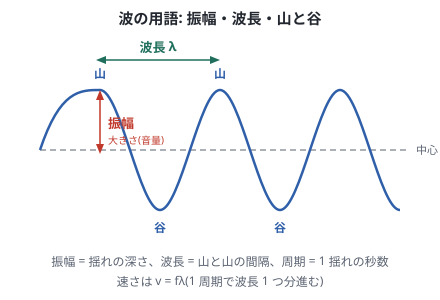
\includegraphics[width=0.85\textwidth]{figures/wave-anatomy.svg}
\caption{波の用語: 振幅・波長・山と谷}
\end{figure}

\subsection{波の 3 つの量: 振幅・周期・波長}

波を数える言葉を 3 つ決めます。

\begin{itemize}
\item \textbf{振幅}: 揺れの深さ(中心から山までの高さ)。大きいほど、エネルギーが大きい。音なら大きさ(音量)、光なら明るさ。
\item \textbf{周期 \( T \)}: 1 回の揺れにかかる秒数。1 秒あたりの揺れの回数を\textbf{振動数 \( f \)} と呼び、\( f = 1/T \) の関係です。音なら高さ(ピッチ)、光なら色。
\item \textbf{波長 \( \lambda \)}: 隣り合う山と山の間隔。波が 1 周期の間に進む距離でもあります。
\end{itemize}

周期と波長をつなぐのが、波の速さの式です。1 周期の間に波長 1 つ分進むのだから、速さは「距離 ÷ 時間」で次のようになります。

\[ v = f \lambda \]

この式は波の分野で最もよく使います。「音が同じでも媒質が変われば速さが変わり、そのとき波長が変わる(振動数は変わらない)」という問題は、この式の読み替えだけで解けます。

\begin{quote}
\textbf{【注意】}\ 波の速さは\textbf{媒質(伝わる物)で決まり、振動数では変わりません}。ギターを強く弾いても音の速さは変わらず、大きさ(振幅)だけが変わります。高く弾いても速さは変わらず、振動数(ピッチ)だけが変わります。速さが変わるのは、空気から水へ、など媒質が変わるときです。
\end{quote}

\textbf{解答の指針:}\ 波の問題では、まず \( v = f\lambda \) の 4 つの量のうち 3 つが分かっているかを確認する。次に、グラフが与えられたら「横軸が時間なら周期を読む問題、横軸が距離なら波長を読む問題」と判別する。2 つのグラフが並んだ問題は、この判別が全てです。振動数は媒質が変わっても不変、速さは媒質で決まる、を図に書き添えておくと混乱しません。

\section{音と光 — 身のまわりの波}

波の道具がそろったので、音と光という 2 大代表を扱います。どちらも \( v = f\lambda \) の世界ですが、性質の違いが試験と実生活の両方で問われます。

\subsection{音: 空気の縦波}

音の速さは空気中で約 340 m/s です。温度で少し変わりますが、高校物理ではこの値を使います。音の\textbf{大きさは振幅}、\textbf{高さ(ピッチ)は振動数}で決まる、という対応をもう一度押さえます。

音の問題で頻出の道具が\textbf{反射(反響)}です。壁に向かって音を出し、跳ね返ってくるまでの時間を測れば、距離は「往復の速さ × 時間 ÷ 2」で出ます。超音波の魚群探知機や、蝙蝠のエコロケーションも同じ計算です。

\textbf{共鳴}も押さえておきます。管の中の空気が、管の長さに合う特定の振動数で大きく振動する現象です。楽器が音を出す仕組みであり、管の長さと波長の関係(閉管なら波長は管の長さの 4 倍、開管なら 2 倍)を式に直す問題が定番です。

\subsection{光: 速さが極大の横波}

光の速さは真空中で約 \( 3.0 \times 10^{8} \) m/s。これほど速いと、身のまわりの距離では時間差を感じませんが、太陽から地球までは約 8 分かかります。つまり私たちが見ている太陽は、8 分前の太陽です。

光は水面やガラスで\textbf{反射}し、別の媒質に入るときに\textbf{屈折}します。屈折は「媒質を変わると速さが変わる」ことで、進む向きが折れ曲がる現象です。ストローが水面で折れて見えるのはこのためです。光の屈折の強さは\textbf{屈折率}で表し、真空の速さに対してその媒質でどれだけ遅くなるかの比です。

\[ n = \frac{c}{v} \]

屈折率が大きいほど光は遅く伝わり、大きく折れ曲がります。水中から水面を見上げると、ある角度を超えた先は水面が鏡のように見える\textbf{全反射}が起こります。光ファイバーは、この全反射で光を端から端まで運ぶ技術です。

\begin{quote}
\textbf{【注意】}\ 音も光も「反射のとき振動数は変わらない」です。反射・屈折で色やピッチが変わることはありません。変わるのは振動数でなく速さと波長のほうです。ドップラー効果(音源と観測者が動くことで音の高さが変わる現象)だけが、観測される振動数を変える特別な場面です。
\end{quote}

\textbf{解答の指針:}\ 音の距離測定では「往復」を忘れないこと(2 で割る)。屈折の問題では、入る前と入った後で振動数が同じまま、\( v = f\lambda \) で速さと波長がどう変わるかを書く。屈折率の式 \( n = c/v \) は「真空の速さを 1 とした、その媒質の遅さの倍率」と読むと、数値の意味を取り違えません。全反射は「密な媒質から疎な媒質へ、浅い角度で入ると起こる」と絵で覚えます。

\section{電気と回路 — 電子の流れを水にたとえる}

最後の場面は電気です。電気は見えないので敬遠されがちですが、\textbf{水の流れにたとえるとほぼ全部が直感に乗ります}。

\subsection{電圧は落差、電流は流量、抵抗は細さ}

水路のたとえで、回路の 3 つの量を対応させます。

\begin{itemize}
\item \textbf{電圧 \( V \)}(単位 V): 電気を押し流す「落差」。高いほど流れが強くなる。電池がこの落差を作ります。
\item \textbf{電流 \( I \)}(単位 A): 1 秒あたりに流れる電気の量。水で言えば流量です。
\item \textbf{抵抗 \( R \)}(単位 \( \Omega \)): 流れにくさ。細い水路は水を流しにくい。電線では、細いほど・材質によっては流れにくい。
\end{itemize}

3 つの量をつなぐのが\textbf{オームの法則}です。落差が 2 倍なら流量も 2 倍、細さが 2 倍なら流量は半分、という関係を 1 式に書いたものです。

\[ V = RI \]

回路図で最もよく使う形は、この式の読み替えです。「抵抗 \( R \) に電圧 \( V \) を掛けたとき流れる電流は \( V/R \)」であり、抵抗の逆数で電流が決まります。

\subsection{直列と並列}

複数の抵抗があるとき、つなぎ方は 2 種類です。

\begin{itemize}
\item \textbf{直列}: 1 本道でつなぐ。水路が長くなるのと同じで、抵抗は\textbf{足し算}。\( R = R_{1} + R_{2} \)。電流はどこでも同じ、電圧は各抵抗で分け合います。
\item \textbf{並列}: 枝分かれさせる。水路が増えるのと同じで、流れやすい。合成抵抗は逆数の足し算。\( 1/R = 1/R_{1} + 1/R_{2} \)。電圧はどの枝でも同じ、電流は枝に分かれます。
\end{itemize}

並列の合成抵抗は、\textbf{どの 1 つの抵抗よりも小さくなる}ことに注意してください。道が増えたのだから流れやすくなる、と水で考えると納得できます。家の電気は、どの部屋でも電圧が同じでなければならないので、すべて並列につながっています。それで、使う電気器具が増えるほど(道が増えるほど)全体の電流が増え、ブレーカーが落ちます。

\begin{figure}
\centering
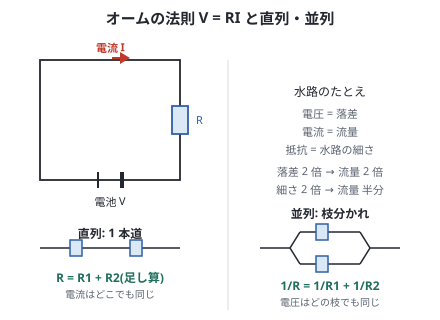
\includegraphics[width=0.85\textwidth]{figures/ohm-circuit.svg}
\caption{オームの法則と直列・並列のつなぎ方}
\end{figure}

\subsection{電力: 流れが仕事をする速さ}

電球が光るのは、電流が抵抗を通るときに仕事をしているからです。1 秒あたりの仕事が\textbf{電力} \( P \) で、単位は W(ワット)。

\[ P = VI = RI^{2} = \frac{V^{2}}{R} \]

3 つの形は、オームの法則で書き換えただけの同じ式です。「100 W の電球を 1 時間使うと 100 Wh の電気料金がかかる」という、電気代の計算もこれが元です。電力会社の「1 kWh」は 1000 W を 1 時間使った分のエネルギーです。

\begin{quote}
\textbf{【注意】}\ 電球に書かれた「100 V・100 W」は\textbf{定格}(その電圧で使ったとき 100 W の仕事をするという設計値)です。実際に掛かる電圧が 50 V なら、\( P = V^{2}/R \) から抵抗一定として電力は 4 分の 1 の 25 W になります。抵抗を先に求めてから、実際の電圧で計算し直すのが定石です。
\end{quote}

\textbf{解答の指針:}\ 回路の問題では、まず「どの抵抗に、どの電圧が掛かり、どの電流が流れるか」を水路の絵で確認する。直列は電流が共通・並列は電圧が共通、この共通の量を軸に立式する。合成抵抗を求める問題では、遠くから順に整理する(並列を 1 つの抵抗にまとめ、それを直列に足す、の繰り返し)。電力は 3 形式を場面で使い分け(電流が分かっているなら \( RI^{2} \)、電圧なら \( V^{2}/R \))、単位の kWh はエネルギー、kW は電力と区別します。

\section{まとめと次の一歩}

10 節を振り返ります。道具は、実は 5 つしかありません。

\begin{itemize}
\item \textbf{単位とベクトル}: 計算の土台。右向き正の宣言を習慣に。
\item \textbf{v-t グラフ}: 傾きが加速度、面積が変位。公式は全部ここから復元できる。
\item \textbf{運動方程式 \( F = ma \)}: 切り離し図に力をすべて書いて 1 本立てる。
\item \textbf{エネルギーと運動量}: 途中の経路が不要な 2 つの道具。衝突は運動量から。
\item \textbf{波と回路の式}: \( v = f\lambda \) と \( V = RI \)。水路のたとえで直感に乗る。
\end{itemize}

やり直し学習で一番効くのは、\textbf{自分で問題を解き直すこと}です。読んだ節について、各節の解答の指針の手順をなぞる形で、1 問ずつでいいので手を動かしてください。物理は「分かった気」になりやすい科目ですが、式を 1 本書けるかどうかで理解の質が全く変わります。

次の一歩としては、この本の先は次のような本へつながります。

\begin{itemize}
\item 加速度の計算をさらに使いたい → \textbf{大学数学入門}(微分が速度と加速度の関係そのものです)
\item 波と振動の数学を見たい → \textbf{フーリエ解析入門}(あらゆる波を音のパレットに分解します)
\item 電気と確率・エネルギーの先にある世界 → \textbf{量子力学の直感}(波の考え方がそのまま生きます)
\item 計算をコンピュータに任せる → \textbf{数値計算入門}(運動方程式をそのままプログラムに書き下します)
\end{itemize}

物理は、絵が描けるかどうかの科目です。この本で描いた絵(切り離し図・v-t グラフ・波の山と谷・水路)を思い出せるうちに、次の本へ進んでください。

\end{document}
